Per quanto riguarda il Training, abbiamo effettuato le stesse scelte effettuate per l'eye detection.

Prima di testare direttamente su Android, anche in questo caso abbiamo deciso prima di testare e analizzare la nostra nuova rete utilizzando la libreria Matplotlib e usando \textbf{Tkinter}.

A fini di testing si è preso ad esempio l'occhio qui sotto:

\begin{figure}[htbp]
    \centering
    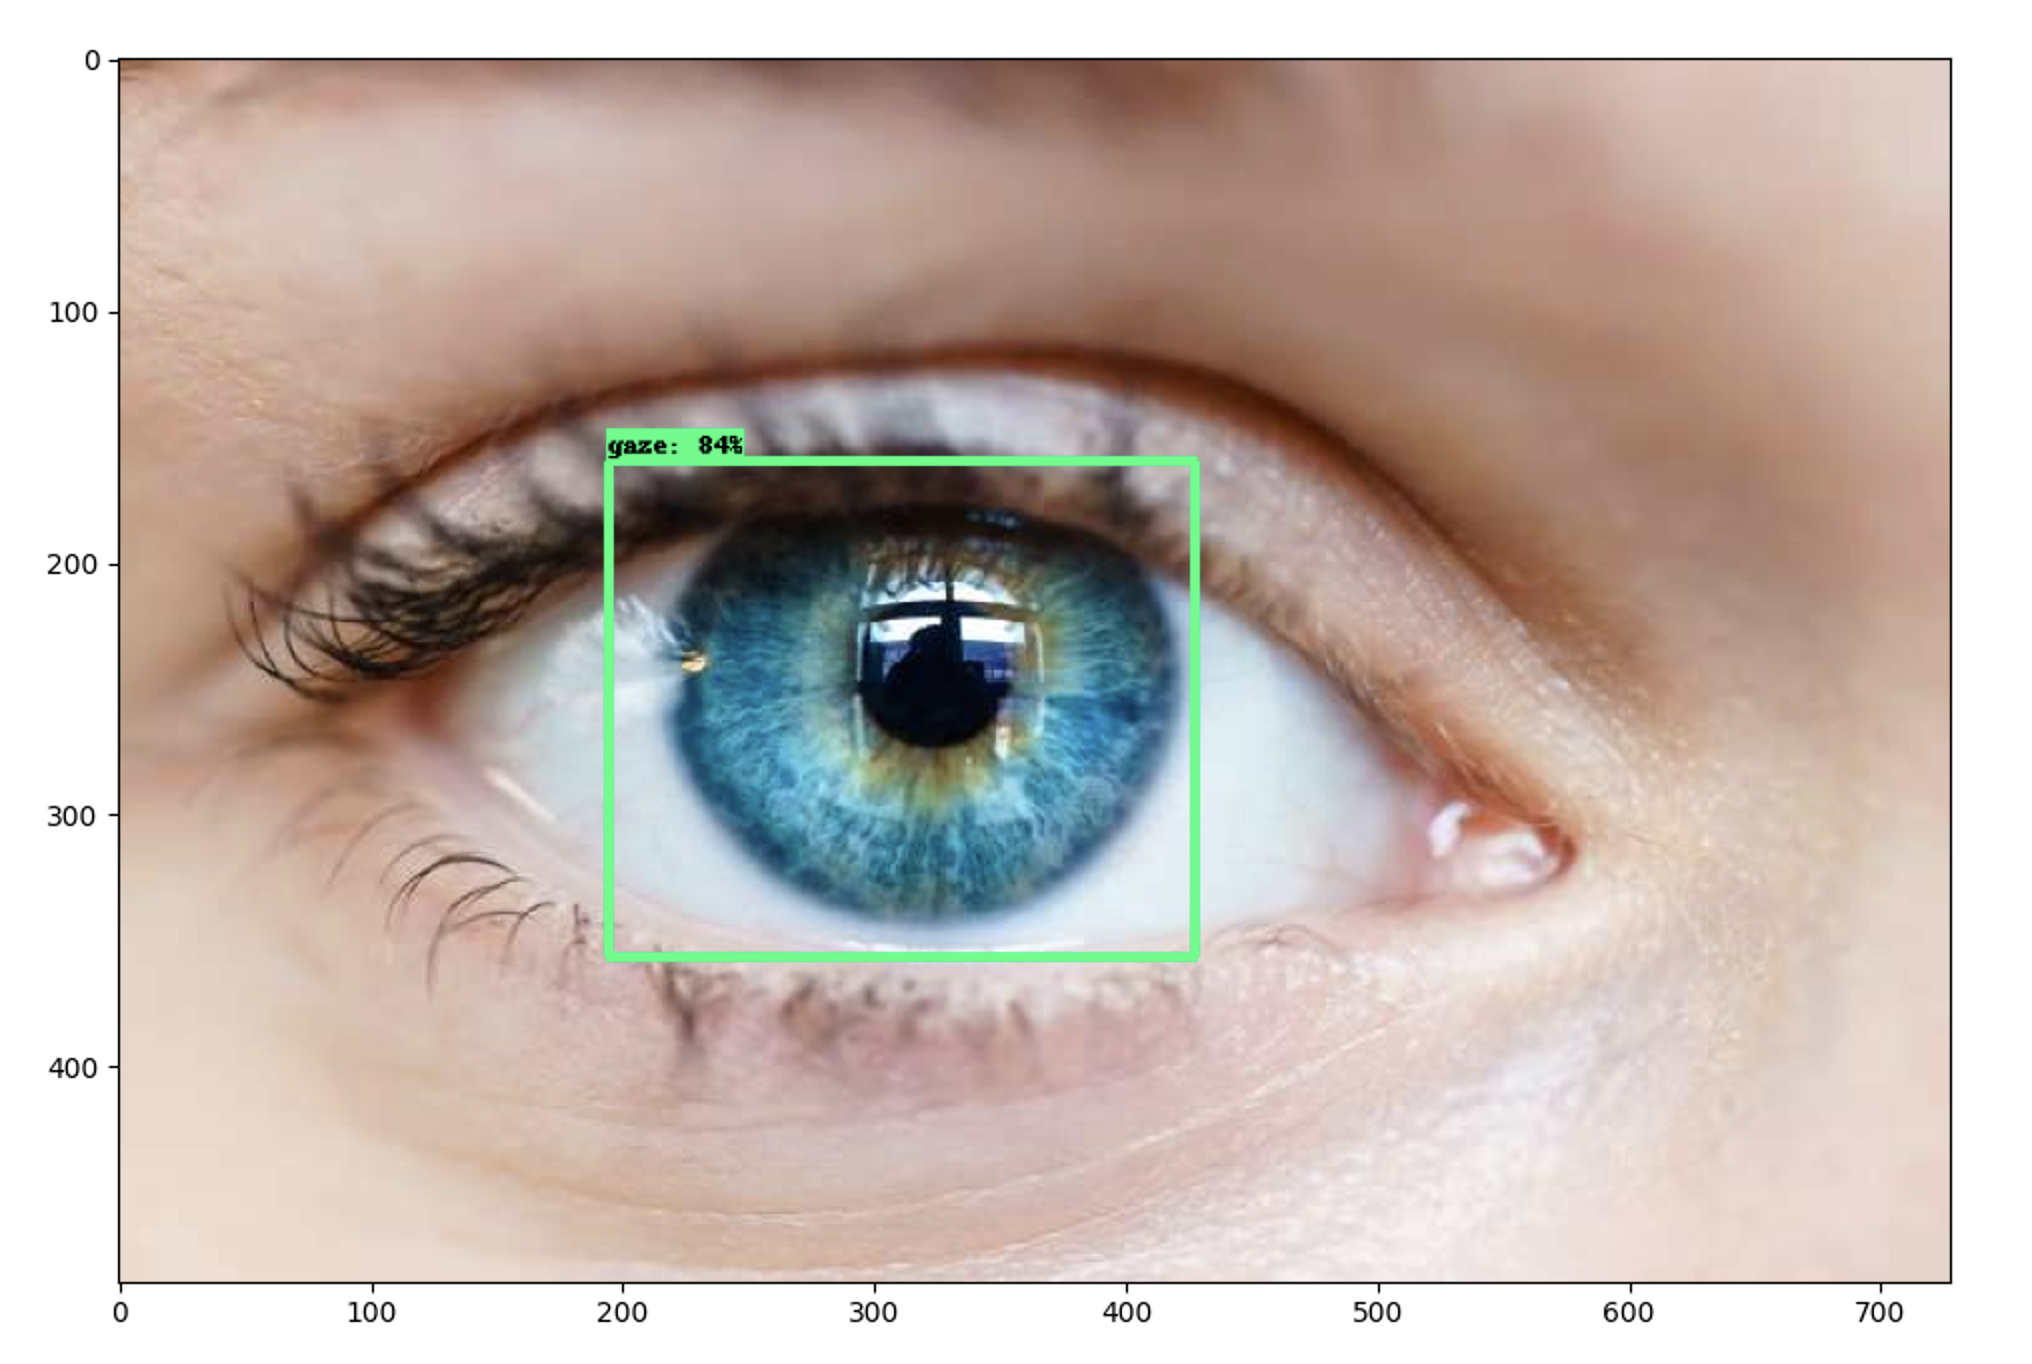
\includegraphics[scale=0.17]{ReteNeurale/PupilDetection/Training/Images/pupilla.png}
    \caption{Test Pupil-Tracking}
    \label{fig:pupil}
\end{figure}